\subsection{逆ラプラス変換と極零点の解釈}

古典制御では、$s$ 領域の式を時間応答へ戻す計算を何度も行う。基本は部分分数分解である。

\begin{formula}[単純極の部分分数分解]
相異なる極 $p_1,\ldots,p_n$ を持つ真にプロパーな伝達関数
\begin{equation}
  F(s)=\frac{N(s)}{(s-p_1)(s-p_2)\cdots(s-p_n)}
\end{equation}
は
\begin{equation}
  F(s)=\sum_{i=1}^{n}\frac{r_i}{s-p_i}
\end{equation}
と書ける。係数 $r_i$ を留数と呼び、
\begin{equation}
  r_i=\lim_{s\to p_i}(s-p_i)F(s)
\end{equation}
で求まる。
\end{formula}

\begin{derivation}
例として
\begin{equation}
  F(s)=\frac{3s+5}{(s+1)(s+4)}
\end{equation}
を考える。部分分数分解を
\begin{equation}
  F(s)=\frac{A}{s+1}+\frac{B}{s+4}
\end{equation}
と置く。通分すると
\begin{equation}
  3s+5=A(s+4)+B(s+1)
\end{equation}
である。$s=-1$ を代入すると
\begin{equation}
  -3+5=A(3)+B(0)
\end{equation}
なので $A=2/3$。$s=-4$ を代入すると
\begin{equation}
  -12+5=A(0)+B(-3)
\end{equation}
なので $B=7/3$。したがって
\begin{equation}
  F(s)=\frac{2/3}{s+1}+\frac{7/3}{s+4}
\end{equation}
であり、逆ラプラス変換は
\begin{equation}
  f(t)=\frac{2}{3}e^{-t}+\frac{7}{3}e^{-4t}
\end{equation}
である。
\end{derivation}

複素共役極 $-\sigma\pm j\omega$ は、時間領域では
\begin{equation}
  e^{-\sigma t}\cos\omega t,
  \qquad
  e^{-\sigma t}\sin\omega t
\end{equation}
の組として現れる。したがって、実部は減衰、虚部は振動を決める。零点は指数成分そのものを新しく作るのではなく、それぞれの指数成分の重みを変える。右半平面零点があると、最終的に正へ動く応答が初めに逆向きへ動くことがある。

\subsection{定常偏差と最終値の定理}

PD 制御は行き過ぎを抑え、振動を減らす。しかし、応答が静かになったあとにも目標値から一定量だけずれていれば、実機では制御できているとは言いにくい。たとえば小さな水槽の水位 $y$ [m] をポンプ入力 $u$ [\%] で保つとき、細い漏れがあると、目標水位 $r$ [m] に止まって見えても常に補給入力が必要になる。偏差 $e=r-y$ [m] に比例する P 制御と、偏差の変化率に比例する D 制御だけでは、定常状態で $\dot{e}=0$ となるため微分項は入力を出さない。必要な補給入力を比例項だけで作るには、$u_\infty=k_\mathrm{P}e_\infty$ となる非零の偏差が残る。

この残り偏差を測定量として見ると、比例ゲインを大きくすれば小さくはなるが、一定外乱がある限り 0 にはならない。積分動作は、この「小さいが消えない偏差」を時間方向に集める状態
\begin{equation}
  \eta(t)=\int_0^t e(\tau)\,d\tau,
  \qquad
  \dot{\eta}=e
\end{equation}
を制御器の内部に持たせる考えである。水位偏差 $e$ の単位が [m] なら、積分状態 $\eta$ の単位は [m\,s] である。入力を
\begin{equation}
  u=k_\mathrm{P}e+k_\mathrm{I}\eta
\end{equation}
とすれば、$k_\mathrm{I}$ の単位は [\%/(m\,s)] であり、偏差が正のあいだ $\eta$ が増え続け、漏れを打ち消すための一定入力を作る。最終的に $e=0$ になれば $\dot{\eta}=0$ となり、積分状態はそこで止まって、必要な補給入力だけを保持する。

\begin{theorem}[最終値の定理]
$sF(s)$ のすべての極が左半平面にあるとき、
\begin{equation}
  \lim_{t\to\infty}f(t)=\lim_{s\to0}sF(s)
\end{equation}
が成り立つ。
\end{theorem}

負帰還で開ループ $L(s)=C(s)G(s)$ とすると、偏差は
\begin{align}
  E(s)&=R(s)-Y(s),\\
  Y(s)&=L(s)E(s).
\end{align}
よって
\begin{align}
  E(s)&=R(s)-L(s)E(s),\\
  \{1+L(s)\}E(s)&=R(s),\\
  E(s)&=\frac{1}{1+L(s)}R(s)=S(s)R(s).
\end{align}
単位ステップ $R(s)=1/s$ に対する定常偏差は、最終値の定理より
\begin{align}
  e_\infty&=\lim_{s\to0}sE(s)\\
  &=\lim_{s\to0}s\frac{1}{1+L(s)}\frac{1}{s}\\
  &=\frac{1}{1+L(0)}.
\end{align}
この計算は、閉ループが安定であり、$sE(s)$ の極が左半平面にある場合にだけ定常値を表す。型 0 のループでは $L(0)$ が有限なので、一定目標や一定外乱に対する残り偏差は有限値として残る。一方、積分器を一つ入れると低周波で $L(s)=\tilde{L}(s)/s$ となり、$\tilde{L}(0)$ が有限正で閉ループが安定なら
\begin{align}
  e_\infty
  &=\lim_{s\to0}\frac{1}{1+\tilde{L}(s)/s}\\
  &=\lim_{s\to0}\frac{s}{s+\tilde{L}(s)}=0
\end{align}
である。これは、積分状態 $\eta$ が漏れや重力分などの一定バイアス入力を保持し、偏差そのものは 0 に近づけられる、という水槽の観察と同じ内容である。

\begin{center}
\begin{tabular}{lll}
\hline
構成 & 低周波の開ループ & 単位ステップ定常偏差 \\
\hline
型 0 & $L(0)=K_p<\infty$ & $1/(1+K_p)$ \\
積分器 1 個 & $L(s)=\tilde{L}(s)/s,\ \tilde{L}(0)>0$ & $0$ \\
\hline
\end{tabular}
\end{center}

\begin{definition}[型と誤差定数]
開ループ $L(s)$ が原点に持つ極の個数を系の型という。位置、速度、加速度誤差定数を
\begin{align}
  K_p&=\lim_{s\to0}L(s),\\
  K_v&=\lim_{s\to0}sL(s),\\
  K_a&=\lim_{s\to0}s^2L(s)
\end{align}
と定義する。
\end{definition}

ステップ、ランプ、放物線入力に対する定常偏差は、閉ループが安定であるという前提のもとで
\begin{align}
  e_{step}&=\frac{1}{1+K_p},\\
  e_{ramp}&=\frac{1}{K_v},\\
  e_{parabolic}&=\frac{1}{K_a}
\end{align}
となる。積分器 $1/s$ を制御器に入れると原点極が一つ増えるため、ステップ偏差を 0 にできる。ただし積分状態は過去の偏差を蓄えるので、むやみに $k_\mathrm{I}$ を大きくすると低周波の補正は強くなる一方で位相遅れも増え、安定余裕は悪くなりやすい。

\subsection{ブロック線図の全経路}

閉ループ評価は目標値応答だけでは不十分である。入力外乱、出力外乱、測定ノイズ、制御入力も同時に評価する必要がある。図\ref{fig:closed-loop-signal-paths} に、同じ負帰還ループでこれらの信号が入る位置を示す。ここでは単位帰還の SISO 系を考え、開ループを $L=CG$、感度を $S=1/(1+L)$、相補感度を $T=L/(1+L)$ とする。

\begin{figure}[tbp]
\centering
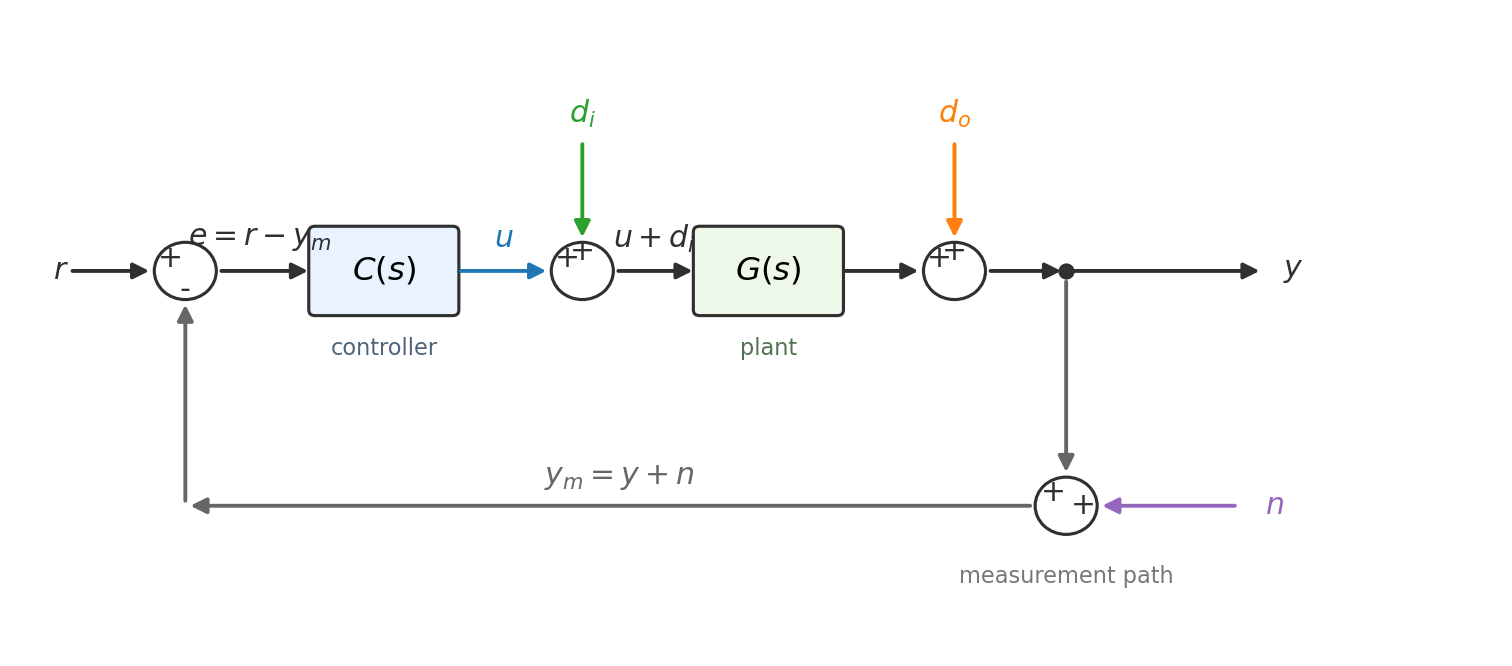
\includegraphics[width=0.96\linewidth,bb=0 0 1512 666]{figures/closed_loop_signal_paths.png}
\caption{目標値 $r$、制御器 $C$、制御対象 $G$、入力外乱 $d_i$、出力外乱 $d_o$、測定ノイズ $n$、制御器出力 $u$、出力 $y$ を含む閉ループの信号経路。入力外乱 $d_i$ は対象入力側に加わるため $GS$ の経路で $y$ を動かし、制御器出力 $u$ にも反作用を生む。出力外乱 $d_o$ は対象後段で $y$ に直接加わり、感度 $S$ で抑えられる。測定ノイズ $n$ は実出力を直接変えず、測定値 $y_m=y+n$ を通じて $-T$ と $-CS$ の経路に入る。$u$ を同時に確認しないと、出力偏差が小さい条件でもアクチュエータ飽和やノイズ増幅を検出できない。}
\label{fig:closed-loop-signal-paths}
\end{figure}

図の符号規約では、入力外乱 $d_i$ が対象入力に加わり、出力外乱 $d_o$ が対象出力の後で加わり、測定ノイズ $n$ は帰還される測定値 $y_m=y+n$ にだけ入る。したがって、すべての入力点を同時に残すと
\begin{align}
  y&=G(u+d_i)+d_o,\\
  u&=C\{r-(y+n)\}
\end{align}
である。代入して整理すると
\begin{align}
  y&=G\{C(r-y-n)+d_i\}+d_o,\\
  y+GCy&=GCr+Gd_i+d_o-GCn,\\
  (1+L)y&=Lr+Gd_i+d_o-Ln.
\end{align}
したがって
\begin{equation}
  y=Tr+GSd_i+Sd_o-Tn.
\end{equation}
目標値だけを入れれば $y=Tr$、入力外乱だけを入れれば $y=GSd_i$、出力外乱だけを入れれば $y=Sd_o$、測定ノイズだけを入れれば $y=-Tn$ である。入力外乱は対象 $G$ を通ってから感度 $S$ で抑えられ、出力外乱は対象の後で加わるため $G$ を通らない。測定ノイズは出力そのものを動かす外力ではないが、帰還信号を誤らせるため相補感度 $T$ を通じて出力に現れる。

制御器出力は
\begin{align}
  u&=C(r-y-n)\\
  &=C\{r-(Tr+GSd_i+Sd_o-Tn)-n\}\\
  &=CSr-CGSd_i-CSd_o-CSn
\end{align}
である。$u$ の式には、外乱を打ち消そうとして制御器がどれだけ大きな指令を出すかが現れる。低周波で $S$ が小さくても、$C$ や $CGS$ が大きい帯域では、外乱補償や測定ノイズのために $u$ が先に飽和することがある。したがって閉ループ設計では、出力 $y$ の小ささだけでなく、制御器出力 $u$、飽和余裕、ノイズ帯域での増幅を同じ条件で確認する。
